\documentclass[letterpaper,10pt]{article}

\usepackage{titling}
\usepackage{listings}
\usepackage{url}
\usepackage{setspace}
\usepackage{subfig}
\usepackage{sectsty}
\usepackage{pdfpages}
\usepackage{colortbl}
\usepackage{multirow}
\usepackage{multicol}
\usepackage{relsize}
\usepackage{amsmath}
\usepackage{fancyvrb}
\usepackage{amsmath,amssymb,amsthm,graphicx,xspace}
\usepackage[titlenotnumbered,noend,noline]{algorithm2e}
\usepackage[compact]{titlesec}
\usepackage{XCharter}
\usepackage[T1]{fontenc}
\usepackage{enumitem}
\usepackage{tikz}
\usetikzlibrary{arrows,automata,shapes,trees,matrix,chains,scopes,positioning,calc}
\tikzstyle{block} = [rectangle, draw, fill=blue!20, 
    text width=2.5em, text centered, rounded corners, minimum height=2em]
\tikzstyle{bw} = [rectangle, draw, fill=blue!20, 
    text width=4em, text centered, rounded corners, minimum height=2em]

\newcommand{\CPP}{C\nolinebreak\hspace{-.05em}\raisebox{.4ex}{\tiny\bf +}\nolinebreak\hspace{-.10em}\raisebox{.4ex}{\tiny\bf +}}
\def\CPP{{C\nolinebreak[4]\hspace{-.05em}\raisebox{.4ex}{\tiny\bf ++}}}

\let\LaTeXtitle\title
\renewcommand{\title}[1]{\LaTeXtitle{\textsf{#1}}}


\addtolength{\oddsidemargin}{-1.000in}
\addtolength{\evensidemargin}{-0.500in}
\addtolength{\textwidth}{2.0in}
\addtolength{\topmargin}{-1.000in}
\addtolength{\textheight}{1.75in}
\addtolength{\parskip}{\baselineskip}
\setlength{\parindent}{0in}
\renewcommand{\baselinestretch}{1.5}

\singlespace


\begin{document}

\lecture{17 --- Critical Paths, Data \& Task Parallelism}{\term}{Patrick Lam}

\section*{Critical Paths}
You should be familiar with the concept of a critical path from previous
courses; it is the minimum amount of time to complete the task, taking
dependencies into account, and without speculating.

Consider the following diagram, which illustrates dependencies between
tasks (shown on the arrows). 
Note that B depends on A, and D depends on B and C, but C does
not depend on anything, so it could be done in parallel with
everything else. You can also compute expected execution times
for different strategies.
\begin{center}
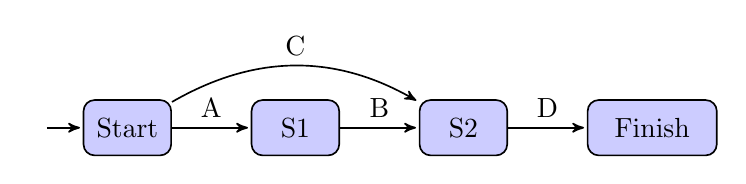
\begin{tikzpicture}[->,>=stealth',shorten >=1pt,auto,column sep=2.2cm,
                    semithick,initial text=]
  \node[initial,block] (s0) {Start};
  \node[block] (s1) [right=of s0] {S1};
  \node[block] (s2) [right=of s1] {S2};
  \node[bw] (s3) [right=of s2] {Finish};

  \path (s0) edge node {A} (s1)
        (s1) edge node {B} (s2)
        (s2) edge node {D} (s3)
        (s0) edge[bend left=30] node {C} (s2);
\end{tikzpicture}
\end{center}

\section*{Data and Task Parallelism}
There are two broad categories of paralellism: data parallelism and
task parallelism. An analogy to data parallelism is hiring a call
center to (incompetently) handle large volumes of support calls,
\emph{all in the same way}. Assembly lines are an analogy to task
parallelism: each worker does a \emph{different} thing.

More precisely, in data parallelism, multiple threads perform the
\emph{same} operation on separate data items. For instance, you have a
big array and want to double all of the elements. Assign part of the
array to each thread. Each thread does the same thing: double array
elements.

In task parallelism, multiple threads perform \emph{different}
operations on separate data items. So you might have a thread that
renders frames and a thread that compresses frames and combines them
into a single movie file.

We'll continue by looking at a number of parallelization patterns,
examples of how to apply them, and situations where they might apply.

\subsection*{Data Parallelism with SIMD}
The ``typical'' boring standard uniprocessor is Single Instruction Single Data (SISD) but since the mid-1980s we've had more options than that. We'll talk about single-instruction multiple-data (SIMD) later on in
this course, but here's a quick look. Each SIMD
instruction operates on an entire vector of data. These instructions
originated with supercomputers in the 70s. More recently, GPUs; the
x86 SSE instructions; the SPARC VIS instructions; and the
Power/PowerPC AltiVec instructions all implement SIMD.

\paragraph{Code.} Let's look at an application of SIMD instructions.

\begin{verbatim}
void vadd(double * restrict a, double * restrict b, int count) {
  for (int i = 0; i < count; i++)
    a[i] += b[i];
}
\end{verbatim}

Compiling this without SIMD on a 32-bit x86 ({\tt gcc -m32 -march=i386 -S}) might give this:
\begin{verbatim}
loop:
  fldl  (%edx)
  faddl (%ecx)
  fstpl (%edx)
  addl  8, %edx
  addl  8, %ecx
  addl  1, %esi
  cmp   %eax, %esi
  jle   loop
\end{verbatim}

We can instead compile to SIMD instructions ({\tt gcc -m32 -march=prescott -mfpmath=sse})
and get something like this:
\begin{verbatim}
loop:
  movupd (%edx),%xmm0
  movupd (%ecx),%xmm1
  addpd  %xmm1,%xmm0
  movpd  %xmm0,(%edx)
  addl   16,%edx
  addl   16,%ecx
  addl   2,%esi
  cmp    %eax,%esi
  jle    loop
\end{verbatim}
The \emph{packed} operations ({\tt p}) operate on multiple data
elements at a time (what kind of parallelism is this?)
The implication is that the loop only needs to loop half as many times.
Also, the instructions themselves are more efficient, because they're
not stack-based x87 instructions.

SIMD is different from the other types of parallelization we're
looking at, since there aren't multiple threads working at once.
It is complementary to using threads, and good for cases
where loops operate over vectors of data. These loops could also be
parallelized; multicore chips can do both, achieving high throughput.
SIMD instructions also work well on small data sets, where thread startup
cost is too high, while registers are just there to use.

We'll see a case study that uses SIMD (also known as vector
instructions) in Lecture 19. In~\cite{lemire18:_multic_simd}, Daniel Lemire argues that vector
instructions are, in general, a more efficient way to parallelize code
than threads. That is, when applicable, they use less overall CPU
resources (cores and power) and can even run faster.

\subsection*{Parallelization using Threads or Processes}
We'll be looking at thread-based or process-based parallelization for the
next bit. We don't care about the distinction between threads and processes
for the moment. In fact, we could even distribute work over multiple systems.

\paragraph{Pattern 1: Multiple Independent Tasks.} If you're just trying to maximize
system utilization, you can use one system to run a number of independent
tasks; for instance, you can put both a web server and database on
one machine. If the web server happens to be memory-bound while the
database is I/O-bound, then both can use system resources. If the web
server isn't talking to the database (rare these days!), then the tasks
would not get in each others' way.

Most services probably ought to be run under virtualization these
days, unless they're trivial or not mission-critical.

A more relevant example of multiple independent tasks occurs in
cluster/grid/cloud computing: the cloud might run a number of
independent tasks, and each node would run some of the tasks. The
cloud can retry a task (on a different node, perhaps) if it fails on
some node. Note that the performance ought to increase linearly with
the number of threads, since there shouldn't be communication between
the tasks.

\paragraph{Pattern 2: Multiple Loosely-Coupled Tasks.} Some applications contain
tasks which aren't quite independent (so there is some inter-task
communication), but not much.  In this case, the tasks may be
different from each other. The communication might be from the tasks
to a controller or status monitor; it would usually be asynchronous or
be limited to exceptional situations.

Refactoring an application this way can help with latency: if you 
split off the CPU-intensive computations into a sub-thread, then
the main thread can respond to user input more quickly.

Here's an example. Assume that an application needs to receive and
forward network packets, and also must log packet activity to disk.
Then the two tasks are clear: receive/forward, and log. Since logging
to disk is a high-latency event, a single-threaded application might
incur latency while writing to disk. Splitting into subtasks allows
the receive/forward to run without waiting for previous packets to be
logged, thus increasing the throughput of the system.

\paragraph{Pattern 3: Multiple Copies of the Same Task.} A common variant of
multiple independent tasks is multiple copies of the same task
(presumably on different data). In this case, we'd require there to be
no communication between the different copies, which would enable
linear speedup. An example is a rendering application running on
multiple distinct animations. We gain throughput, but need to wait
just as long for each task to complete.

\paragraph{Pattern 4: Single Task, Multiple Threads.} This is the classic
vision of ``parallelization'': for instance, distribute array
processing over multiple threads, and let each thread compute the
results for a subset of the array.

This pattern, unlike many of the others before it, can actually
decrease the time needed to complete a unit of work, since it gets
multiple threads involved in doing the single unit simultaneously.
The result is improved latency and therefore increased throughput.
Communication can be a problem, if the data is not nicely
array-structured, or has dependencies between different array parts.

Other names and variations for this pattern include ``fork-join'',
where the main process forks its execution and gives work to all of
the threads, with the join synchronizing threads and combining the
results; and ``divide-and-conquer'', where a thread spawns subthreads
to compute smaller and smaller parts of the solution.

\paragraph{Pattern 5: Pipeline of Tasks.} We've seen pipelining in the context of
computer architecture. It can also work for software. For instance,
you can use pipelining for packet-handling software, where multiple
threads, as above, might confound the order. If you use a three-stage
pipeline, then you can have three packets in-flight at the same time,
and you can improve throughput by a factor of 3 (given appropriate
hardware).  Latency would tend to remain the same or be worse (due to
communication overhead).

Some notes and variations on the pipeline: 1) if a stage is
particularly slow, then it can limit the performance of the entire
pipeline, if all of the work has to go through that stage; and 2) you
can duplicate pipeline stages, if you know that a particular stage is
going to be the bottleneck.

\paragraph{Pattern 6: Client-Server.} Botnets work this way (as does \verb+SETI@Home+,
etc). To execute some large computation, a server is ready to tell
clients what to do.  Clients ask the server for some work, and the
server gives work to the clients, who report back the results. Note
that the server doesn't need to know the identity of the clients for
this to work.

A single-machine example is a GUI application where the server part
does the backend, while the client part contains the user interface.
One could imagine symbolic algebra software being designed that way.
Window redraws are an obvious candidate for tasks to run on clients.

Note that the single server can arbitrate access to shared resources.
For instance, the clients might all need to perform network access.
The server can store all of the requests and send them out in an
orderly fashion.

The client-server pattern enables different threads to share work
which can somehow be parcelled up, potentially improving
throughput. Typically, the parallelism is somewhere between single
task, multiple threads and multiple loosely-coupled tasks. It's also a
design pattern that's easy to reason about.

\paragraph{Pattern 7: Producer-Consumer.} The producer-consumer is 
a variant on the pipeline and client-server models. In this case, the
producer generates work, and the consumer performs work. An example is
a producer which generates rendered frames, and a consumer which
orders these frames and writes them to disk. There can be any number
of producers and consumers. This approach can improve throughput
and also reduces design complexity.

\paragraph{Combining Strategies.} If one of the patterns suffices,
then you're done. Otherwise, you may need to combine strategies.
For instance, you might often start with a pipeline, and then 
use multiple threads in a particular pipeline stage to handle one
piece of data. Or, as I alluded to earlier, you can replicate
pipeline stages to handle different data items simultaneously.

Note also that you can get synergies between different patterns.
For instance, consider a task which takes 100 seconds. First, you
take 80 seconds and parallelize it 4 ways (so, 20 seconds). This
reduces the runtime to 40 seconds. Then, you can take the serial 
20 seconds and split it into two threads. This further reduces 
runtime to 30 seconds. You get a $2.5\times$ speedup from the
first transformation and $1.3\times$ from the second, if you do it
after the first. But, if you only did the second parallelization,
you'd only get a $1.1\times$ speedup.

\subsection*{How to Parallelize Code}
Here's a four-step outline of what you need to do.
\begin{enumerate}
\item Profile the code.
\item Find dependencies in hotspots. For each dependency chain in
a hotspot, figure out if you can execute the chain as
multiple parallel tasks or a loop over multiple parallel iterations.
Think about changing the algorithm, if that would help.
\item Estimate benefits. 
\item If they're not good enough (e.g. far from linear speedup),
step back and see if you can parallelize something else up the
call chain, or at a higher level of absraction.
(Think Mandelbrot sets and computing different points in parallel).
\end{enumerate}
Try to reduce the amount of synchronization that you have to do
(waiting for parallel tasks to finish), because that always slows
you down.

\section*{Thread Pools} We talked about ``single task, multiple threads''
above. The idea behind a \emph{thread pool} is that it's relatively
expensive to start a thread; it costs resources to keep the threads
running at the operating system level; and the threads won't run
optimally anyway, because they'll spend too much time swapping state
in and out of the cache.  Instead, you start an appropriate number of
threads, which each grab work from a work queue, do the work,
and report the results back. Web servers are a good application of
thread pools\footnote{Apache does this: \url{http://httpd.apache.org/docs/2.0/mod/worker.html}. Also see an assignment where the students write thread-pooled web servers: \url{http://www.cse.nd.edu/~dthain/courses/cse30341/spring2009/project4/project4.html}.}.

A key question is: how many threads should you create?  This depends
on which resources your threads use; if you are writing
computationally-intensive threads, then you probably want to have
fewer threads than the number of virtual CPUs. You can also use
Amdahl's Law to estimate the maximum useful number of threads, as
discussed previously.

Here's a longer discussion of thread pools:

\begin{center}
\url{http://www.ibm.com/developerworks/library/j-jtp0730.html}
\end{center}

Modern languages provide thread pools; Java's
\url{java.util.concurrent.ThreadPoolExecutor}~\cite{java:threadpoolexecutor}, C\#'s
\url{System.Threading.ThreadPool}~\cite{csharp:threadpool}, and GLib's {\tt GThreadPool}~\cite{gnome:threadpool} all implement thread pools. 

\paragraph{GLib.} 
GLib is a C library developed by the GTK team. It provides many useful
features that you might otherwise have to implement yourself in C.
%Consider using GLib's thread pool in your assignment 2, unless you
%want to implement the work queue yourself.  (I see no reason to do
%that!)

\bibliographystyle{alpha}
\bibliography{459}


\end{document}
